\begin{figure}[tbp]
  \centering
  \begingroup
  \definecolor{turnblue}{RGB}{48,91,120}
  \definecolor{turnorange}{RGB}{163,92,43}
  \resizebox{0.95\linewidth}{!}{%
  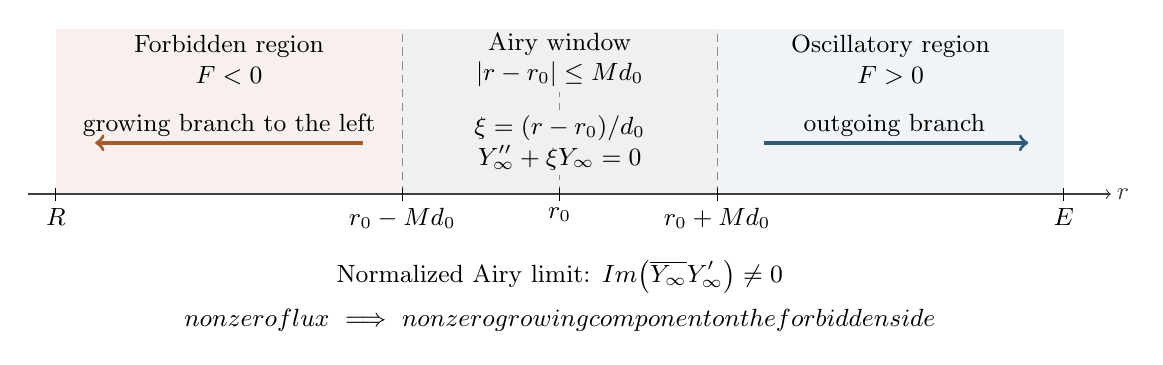
\begin{tikzpicture}[
    x=1cm,y=1cm,font=\small,
    guide/.style={densely dashed,thin,black!45},
    every node/.style={inner sep=2pt}]
    \fill[turnorange!9] (.6,0) rectangle (5,2.1);
    \fill[black!6] (5,0) rectangle (9,2.1);
    \fill[turnblue!7] (9,0) rectangle (13.4,2.1);
    \draw[guide] (5,0) -- (5,2.1);
    \draw[guide] (9,0) -- (9,2.1);
    \draw[guide] (7,0) -- (7,1.3);
    \node[align=center] at (2.8,1.7) {Forbidden region\\$F<0$};
    \node[align=center] at (7,1.7) {Airy window\\$|r-r_0|\le M d_0$};
    \node[align=center] at (11.2,1.7) {Oscillatory region\\$F>0$};
    \draw[<-,very thick,turnorange] (1.1,.65) -- (4.5,.65);
    \node[above] at (2.8,.65) {growing branch to the left};
    \node[align=center,fill=black!6] at (7,.65) {$\xi=(r-r_0)/d_0$\\$Y_\infty''+\xi Y_\infty=0$};
    \draw[->,very thick,turnblue] (9.6,.65) -- (12.95,.65);
    \node[above] at (11.25,.65) {outgoing branch};
    \draw[->,thin,black!75] (.25,0) -- (14,0) node[right] {$r$};
    \foreach \x in {.6,5,7,9,13.4}
      \draw (\x,.08) -- (\x,-.09);
    \node[below] at (.6,-.1) {$R$};
    \node[below] at (5,-.1) {$r_0-Md_0$};
    \node[below] at (7,-.1) {$r_0$};
    \node[below] at (9,-.1) {$r_0+Md_0$};
    \node[below] at (13.4,-.1) {$E$};
    \node[align=center] at (7,-1.05)
      {Normalized Airy limit: $\displaystyle
       \operatorname{Im}\!\left(\overline{Y_\infty}Y_\infty'\right)\ne0$};
    \node[align=center] at (7,-1.6)
      {$\text{nonzero flux}\ \Longrightarrow\ \text{nonzero growing component on the forbidden side}$};
  \end{tikzpicture}%
  }
  \endgroup
  \caption{Schematic of a channel with one turning point in the
  high-parameter estimate, with $R\in[B_0,B_1]$ as in
  Lemma~\ref{spec:scalar-turn}. The scalar solution is selected at $E$ by
  $U(E)=F(E)^{-1/4}$ and $U'(E)=h i\sqrt{F(E)}\,U(E)$.
  For a fixed large $M$, pass to a subsequence and take the
  high-parameter limit in the window using $Y=d_0^{-1/2}U$
  and $\xi=(r-r_0)/d_0$.
  The resulting Airy solution has constant nonzero flux, so it contains
  a branch growing towards $R$.
  Only after this fixed-window limit is $M$ allowed to tend to infinity
  to obtain the normalized logarithmic derivative
  $U'(R)/(\sqrt{-F(R)}\,U(R))\to-1$.
  Distances are not to scale, and the arrows indicate branch selection,
  not a graph of $U$ or a sign assertion for its complex values.}
  \label{fig:turning}
\end{figure}
